% -*- mode: fundamental -*-

% ****************************************************************

\chapter{BSV: Overview of the BSV program structure}

\markboth{Ch \arabic{chapter}: BSV: Packages}{\copyrightnotice}

\setcounter{page}{1}
% \renewcommand{\thepage}{\arabic{page}}
\renewcommand{\thepage}{\arabic{chapter}-\arabic{page}}

\label{ch_Packages}

% ****************************************************************

\section{Introduction}

In this chapter we describe the top-level view of a BSV program.  The
goal is to quickly develop an ability to scan BSV code (from Fife or
Drum or any other example) and to discern the structure and
relationships of the components in the code.

At the syntactic level, a BSV design can be organized into multiple
source files, each containing a BSV ``\verb|package|''.  Packages
contain top-level definitions of types, values, functions, interfaces
and modules.  The names of these entities are local to the package.
Components defined in one package are visible in other packages using
an ``\verb|import|'' statement.

At the semantic level, a BSV design is organized into hardware
``\verb|module|s''.  Each module presents, to the outside world (the
environment), an ``\verb|interface|'' containing ``\verb|method|s'',
which constitute the API by which the environment interacts with the
module.

A module may contain ``\verb|rule|s'' which are independent processes.
It can invoke instances of other modules by invoking their interface
methods.

The sections of this chapter present an overview of these major
components, after first showing a simple (even trivial) example BSV
program.

% ****************************************************************

\section{A Minimal BSV program}

Here is a minimal complete BSV program (although it is not very
interesting as hardware!).

\index[BSV]{\$display@{\tt \$display} statements}

{\small
\begin{Verbatim}[frame=single, numbers=left, label=in file Exercises/Ex\_03\_A\_Hello\_World/Top.bsv]
module mkTop (Empty);

   rule rl_once;
      $display ("Hello, World!");
      $finish (0);
   endrule
      
endmodule
\end{Verbatim}
}

It defines one module, \verb|mkTop|, with an \verb|Empty| interface,
{\ie} a module with no inputs or outputs (we will discuss modules and
interfaces in more detail later).  The module contains one rule,
\verb|rl_once|, whose rule body contains two statements, a
\verb|$display()| statement/expression that prints the message and a
\verb|$finish(0)| statement/expression which terminates the simulation
immediately, returning an exit value of 0 to the operating system.
Rules can normally execute repeatedly forever, but here the
\verb|$finish()| terminates it after one execution (rules are
discussed in more detail in Chapters~\ref{ch_Rules_I} and
Chapters~\ref{ch_Rules_II}).

% ----------------
\vspace{1ex}

NOTE:
\fbox{\small
\begin{minipage}{5in}

{\tt \$display()} is only meaningful in simulation, where the
simulator can print out characters to the terminal in which the
simulation is running.  Actual hardware may or may not have any
terminal at all.  Some hardware may have a UART (Universal
Asynchronous Receiver/Transmitter) that can send characters to a
terminal.  For this, the CPU must run a RISC-V program that sends the
characters, one by one, to the terminal.

\vspace{1ex}

{\tt \$finish()} is only meaningful in simulation, where the
simulation is a program running under some operating system (Linux,
Windows, MacOS, ...) and it is meaningful to ``terminate'' the
simulation and return to a command-line with an exit value.  Actual
hardware has no concept of ``terminating'', it just runs forever as
long as it is supplied power and a clock signal.

\end{minipage}}

\vspace{1ex}
% ----------------

We can simulate in Bluesim or in Verilog simulation; in both cases it
just prints ``Hello World!'' and exits.  For Bluesim, we can compile
and link it using the free and open-source \emph{bsc} compiler, and
then run the executable:

{\small
\begin{Verbatim}[frame=single, numbers=left]
  $ bsc -sim  -g mkTop  Top.bsv                          # compile
  $ bsc -sim  -e mkTop  -o exe_HW_bsim                   # link
  $ ./exe_HW_bsim                                        # run
  Hello, World!                                          # output
\end{Verbatim}
}

We can compile it to Verilog, then compile the Verilog and link it for
Verilog simulation using the free and open-source \emph{verilator}
compiler, and then run the executable:

{\small
\begin{Verbatim}[frame=single, numbers=left]
  $ bsc -verilog  -g mkTop  Top.bsv                      # compile -> mkTop.v
  $ bsc -vsim verilator  -e mkTop  -o exe_HW_vsim        # link
  $ ./exe_HW_vsim                                        # run
  Hello, World!                                          # output
  - mkTop.v:41: Verilog $finish
\end{Verbatim}
}

In both the Bluesim and Verilator cases, the ``\verb|-g|'' flag tells
\emph{bsc} the name of the top-level module for which to generate
code, ``\verb|-e|'' tells it which is the top-level module for
simulation, and ``\verb|-e|'' tells it the desired name for the final
executable.

In Bluesim compile-link, ``\verb|-sim|'' tells \emph{bsim} that our
target is Bluesim.

In Verilog compile-link, ``\verb|-verilog|'' tells \emph{bsim} to
generate Verilog, and it produces the Verilog file \verb|mkTop.v|.
The ``\verb|-vsim|'' flag tells \emph{bsc} to use the Verilator
compiler to compile the generated Verilog into a Verilog simulation
executable.

% ----------------------------------------------------------------
\Beginexercise

Please see directory: \hm {\tt Exercises/Ex\_03\_A\_Hello\_World/} \\
and its README.
\Endexercise

% ================================================================

\subsection{More about {\tt \$display}()}

\label{BSV_display}

The \verb|$display()| function in {\BSV} is similar to
\verb|$display()| in Verilog and SystemVerilog, and to \verb|printf()|
in C/C++. The first argument is a string containing formatting
directives for the remaining arguments. Example:

{\small
\begin{Verbatim}[frame=single, numbers=left]
      Bit #(4) a = 'b_1010;
      Bit #(4) b = 'b_0110;

      $display ("  %04b %04b => %d", a, b, a == b);
\end{Verbatim}
}

The {\tt a} and {\tt b} arguments to \verb|$display()| are printed in
binary format using 4-characters, prefixing it, if necessary, with the
``0'' character.

The {\tt a==b} argument is an expression whose value is of type {\tt
Bool} (Section~\ref{Sec_BSV_Boolean_values}).  Here, we are printing
its bit-representation with the ``\verb|%d|'' format (decimal
integer), so it will print ``0'' for \verb|False| and ``1'' for
\verb|True|.

{\BSV}'s \verb|$display()| goes beyond SystemVerilog's
\verb|$display()| in that arguments can can also be of type \verb|Fmt|
which are computed formatted objects created by the \verb|fshow()|
function which is predefined on all the standard types including
\verb|Bool|.  In our example, we can have it print the \emph{words}
\verb|False| and \verb|True| instead of ``0'' and ``1'' by using
\verb|fshow()|; in this case we omit the ``\verb|%d|'' from the format
string:

{\small
\begin{Verbatim}[frame=single]
      ...
      $display ("  %04b %04b => ", a, b, fshow (a == b));
      ...
\end{Verbatim}
}

The use of \verb|Fmt| and \verb|fshow()| is discussed in more detail
in Section~\ref{Sec_display_and_fmt}.

% ****************************************************************

\section{Packages and files}

\index[BSV]{package@{\tt package}}
\index[BSV]{endpackage@{\tt endpackage}}

Like many programming languages, BSV has facilities to organize large
programs into separately compilable, purposeful, reusable parts.  A
BSV program may be organized into one or more \emph{files} or
\emph{packages}.  This is illustrated in
Figure~\ref{Fig_BSV_program_structure}.
\begin{figure}[htbp]
  \centerline{\includegraphics[width=6in,angle=0]{Figures/Fig_BSV_program_structure}}
  \caption{\label{Fig_BSV_program_structure}
           File-level view of a BSV program}
\end{figure}

A package can contain a number of top-level statements (more detail
about this in Section~\ref{Sec_package_contents}).  One kind of
top-level statment is the ``\verb|import|'' statement, illustrated in
the diagram.  This allows an importing package $p_1$ to use all the
identifiers exported by a package $p_2$ (in addition to indentifiers
defined in $p_1$ itself).

There is a one-to-one correspondence between files and packages.  In
each import statements in the diagram we provide a package name $p$;
the \emph{bsc} compiler uses the imported package name $p$ to find a
file called $p$\verb|.bsv| containing the definition of package $p$.

% ================================================================

\subsection{What's in a Package?}

\label{Sec_package_contents}

Figure~\ref{Fig_BSV_Package} illustrates the typical
structure and contents of a package/file.
\begin{figure}[htbp]
  \centerline{\includegraphics[width=6in,angle=0]{Figures/Fig_BSV_Package}}
  \caption{\label{Fig_BSV_Package}
           What's in a BSV package/file?}
\end{figure}

The \verb|package|--\verb|endpackage| keywords bracketing the
text---the first and last items in the file---are optional; if
omitted, the \emph{bsc} compiler will implicitly create a package name
using the file name.  We recommend always to use
\verb|package|--\verb|endpackage|, except perhaps for small,
experimental, one-off programs to test some small concept.

At the top-level of a package we find import/export statements, type
declarations, value definitions, function definitions interface
declarations and module definitions.

Import/export statements and type and interface declarations are only
allowed at the top-level of a package and not inside any nested
scopes.  An interface declaration is just a kind of type declaration;
its declared interface identifier is used just like a type.

Value, function and module definitions appear at package top-level,
but can also be inside nested scopes (inside function and module
definitions, or other local scopes like \verb|begin|--\verb|end| and
\verb|action|--\verb|endaction| blocks).  Function and module
definitions are, in fact, just value definitions of functional and
module type, respectively.

The top-to-bottom order of entities in a package is not important,
just that if an entity $x$ is defined in the package and used by
another entity $y$ in the same package, then $x$ should be given
before $y$.  We typically place import/export statements at the top of
the file.

Each package/file is separately compiled by the \emph{bsc} compiler,
which saves information about the compilation so that it won't be
recompiled unless the source file has subsequently been modified.

\hdivider

% ----------------------------------------------------------------

\subsection{Extending our example minimal BSV program}

Let us extend our minimal BSV program into one that is split into two
packages/files.  We create a new file \verb|DUT.bsv| that just defines
some top-level scalar constants (strings, bit-vectors).

{\small
\begin{Verbatim}[frame=single, numbers=left, label=in file Ex\_04\_02/DUT.bsv]
package DUT;

String title   = "The C Programming Language";
String authors = "Kernighan and Ritchie";

Bit #(11) year = 1978;

Bit #(4)  month = 2;

Bit #(5)  day = 22;

endpackage
\end{Verbatim}
}

The first and last lines specify that this is a package called
\verb|DUT|.  This was not strictly necessary since \emph{bsc} will use
the package name \verb|DUT| anyway from the filename \verb|DUT.bsv|,
but we prefer always to have package names in our files.

In each line we have a \emph{type}, a
\emph{variable}/\emph{identifier}/\emph{name}, and a value; it
declares the variable to have that type and that value.

Next, we extend our \verb|mkTop| module from the previous example:

{\small
\begin{Verbatim}[frame=single, numbers=left, label=in file Ex\_04\_02/Top.bsv]
package Top;

import DUT :: *;

module mkTop (Empty);

   rule rl_once;
      $display ("Hello, World!");
      $display ("  (From the book: %s", title);
      $display ("   which was first published on: %4d-%02d-%02d)",
                year, month, day);
      $finish (0);
   endrule

endmodule

endpackage
\end{Verbatim}
}

We have explicitly named the package \verb|Top|.  We \verb|import| the
\verb|DUT| package so we can use the variables/identifiers/names
defined in that package.  In the rule, we have added two more
\verb|$display()| statements to print values from the \verb|DUT|
package.

We can compile and link it for Bluesim using the \emph{bsc} compiler,
and then run the executable:

{\small
\begin{Verbatim}[frame=single, numbers=left]
  $ bsc  -u  -sim  -g mkTop  Top.bsv                     # compile
  $ bsc  -sim  -e mkTop  -o exe_HW_bsim                  # link
  $ ./exe_HW_bsim                                        # run
  Hello, World!                                          # output
    (From the book: The C Programming Language
     by:            Kernighan and Ritchie
     which was first published on: 1978-02-22)
\end{Verbatim}
}

We can compile it to Verilog, then compile the Verilog and link it for
Verilog simulation using the \emph{verilator} compiler, and then run
the executable:

{\small
\begin{Verbatim}[frame=single, numbers=left]
  $ bsc -u  -verilog  -g mkTop  Top.bsv                  # compile -> mkTop.v
  $ bsc -vsim verilator  -e mkTop  -o exe_HW_vsim        # link
  $ ./exe_HW_vsim                                        # run
  Hello, World!                                          # output
    (From the book: The C Programming Language
     by:            Kernighan and Ritchie
     which was first published on: 1978-02-22)
  - mkTop.v:47: Verilog $finish
\end{Verbatim}
}

In both, for the compile step, we added the ``\verb|-u|'' flag, which
tells \emph{bsc} to automatically compile any imported files.  This is
why we never had to mention the \verb|DUT.bsv| source file in the
above commands.

% ----------------------------------------------------------------
\Beginexercise

Please see directory: \hm {\tt Exercises/Ex\_03\_B\_Top\_and\_DUT/} \\
and its README.
\Endexercise
% ----------------------------------------------------------------

% ----------------
\vspace{2ex}

NOTE:
\fbox{\small
\begin{minipage}{5in}

From this point on we are not going to show the compile-and-link steps
for each example.  Please consult the \emph{Bluespec Compiler (BSC)
User Guide}~\cite{bsc_user_guide} for full details on how to use the
\emph{bsc} compiler.

\end{minipage}}
% ----------------

% ================================================================

\subsection{Visibility of names, exports and imports}

The \verb|package|, \verb|import| and \verb|export| statements work
just like in SystemVerilog (in fact, using the same syntax).  The
\verb|export| and \verb|import| statements control visibility of names
across packages.  This is illustrated in Figure~\ref{Fig_BSV_namespace_control}.
\begin{figure}[htbp]
  \centerline{\includegraphics[width=6in,angle=0]{Figures/Fig_BSV_namespace_control}}
  \caption{\label{Fig_BSV_namespace_control}
           Namespace control with imports and exports}
\end{figure}

\index[BSV]{export@{\tt export} statement}
\index[BSV]{import@{\tt export} statement}

A package \verb|P| that defines a name $x$ can make it visible outside
using an \verb|export| statement.  As a shorthand, if there is no
\verb|export| statement, then \emph{all} the names defined in a
package are made visible outside.  For convenient readability, if
there are many explicitly exported names, they can be provided using
multiple \verb|export| statements.

A package \verb|Glurph| can also \emph{re-export} names it has
imported from some other package \verb|Phrym|.

If a package \verb|Phoux| needs to use a name \verb|x| defined in some
other package \verb|Baz|, it must explicitly ``\verb|import|'' the
package with the syntax:

{\small
\begin{Verbatim}[frame=single]
import Baz :: *;
\end{Verbatim}
}

which makes all the names exported by \verb|Baz| available for use in
\verb|Phoux|.

% ----------------
\vspace{2ex}

NOTE:
\fbox{\small
\begin{minipage}{5in}

In SystemVerilog, in {\tt import} statement, instead of ``{\tt *}''
one can list just the names actually needed, one does not have to
import all the names exported by another package.  This selective
import is not currently supported in BSV.

\end{minipage}}
% ----------------

% ================================================================

\subsection{Resolving ambiguous imports}

\index[BSV]{Fully-qualified imported names}

If a package \verb|Phoux| imports two other packages \verb|Baz| and
\verb|Glurph|, and both those packages define an identifier \verb|x|,
then the identifier \verb|x| is ambiguous in \verb|Phoux|.  This can
always be resolved by replacing any use of \verb|x| in \verb|Phoux| by
a so-called \emph{fully qualified name}, \verb|Baz::x| or
\verb|Glurph::x| to identify exactly which \verb|x| is intended.

% ================================================================

\subsection{Exporting types abstractly}

\index[BSV]{Exporting types abstractly}

When exporting a struct type \verb|S| or enum type \verb|E| using
\verb|export|, there is a difference between these two ways of
exporting:

\begin{center}
 \begin{tabular}{ccc}
  {\tt export S (..);} & \hmm {\vs} \hmm & {\tt export S;} \\
  {\tt export E (..);} & \hmm {\vs} \hmm & {\tt export E;}
 \end{tabular}
\end{center}

In the versions on the left the field names of the struct and the
labels of the enum are also made visible; on the right, they are not.
The latter case useful in defining a so-called ``\emph{abtract data
type}'', {\ie} a type that is known outside the package but whose
internal details are hidden.

Since an interface is just like a struct type, if we explicitly export
it we typically use:

\begin{center}
\mbox{\tt export M\_IFC (..);}
\end{center}

since we normally want all the interface methods in the interface to
be visible.

% ****************************************************************

\section{Interface and Module Declarations}

\label{Sec_Interface_and_Module_decls}

\index[BSV]{module!declaration}
\index[BSV]{interface!declaration}

% ----------------------------------------------------------------

\subsection{What's in an interface declaration?}

\label{Sec_Whats_in_an_interface_declaration}

\index[BSV]{interface@{\tt interface}!declaration (a module's API)!typical components in}

A BSV interface declaration can appear as a top-level declaration in a
package.  It is a syntactic specification of the ``API'' (Application
Programming Interface) of one or more BSV modules, {\ie} it names the
\emph{methods} offered by a module, and their arguments and result
types.  Figure~\ref{Fig_BSV_whats_in_an_interface_decl} shows examples
of what one might find in an interface declaration (a top-level
declaration inside a package).
\begin{figure}[htbp]
  \centerline{\includegraphics[width=6in,angle=0]{Figures/Fig_BSV_whats_in_an_interface_decl}}
  \caption{\label{Fig_BSV_whats_in_an_interface_decl}
           Typical components in an interface declaration}
\end{figure}

The example declaration introduces a new interface type,
\verb|Baz_IFC|.  Interface types may or may not have type parameters;
the example shows two.  Each type parameter can be of ``numeric'' type
or ordinary ``value'' type.  Numeric types are typically used for
``sizes''; for example, the type ``\verb|Bit#(16)|'' applies the type
constructor ``\verb|Bit|'' to the numeric type ``\verb|16|'' to
describe the type of bit-vectors of width 16 bits.

In places where we \emph{use} this newly declared interface type, it
may look something like this: \verb|Baz_IFC#(3,Bool)|.

The order in which the method/sub-interface declarations are given is
not important.

Some syntax notes for Figure~\ref{Fig_BSV_whats_in_an_interface_decl}:
\begin{tightlist}

 \item Syntax keywords: \verb|interface|, \verb|endinterface|,
       \verb|method|, \verb|numeric|, \verb|type|

 \item Type names (begin with an uppercase letter):
  \begin{tightlist}

   \item \verb|Action|, \verb|ActionValue|, \verb|Bit|, \verb|Int|,
         \verb|Bool| (all standard types in the \emph{bsc} library)

   \item \verb|FIFO_O| (defined in an additional BSV library,
          and discussed in Section~\ref{Sec_Semi_FIFOs})
  \end{tightlist}

 \item Type variables (begin with a lower case letter): \verb|n|, \verb|t|

 \item Ordinary variables (begin with a lower case letter): \verb|m1|,
       \verb|x|, \verb|y|, \verb|z|, \verb|m2|, \verb|m3|,
       \verb|fo_tags|

\end{tightlist}

% ----------------------------------------------------------------

\subsection{What's in a module declaration?}

\label{Sec_Whats_in_a_module_declaration}

\index[BSV]{module@{\tt module}!declaration!typical components in}

A module declaration specifies one of possibly many
\emph{implementations} of a module interface.  If we think of an
interface type as an API, then a module declaration describes an
object (an actual circuit in hardware) that offers that interface.
Figure~\ref{Fig_BSV_whats_in_a_module_decl} shows the typical contents
of a module declaration.
\begin{figure}[htbp]
  \centerline{\includegraphics[width=6in,angle=0]{Figures/Fig_BSV_whats_in_a_module_decl}}
  \caption{\label{Fig_BSV_whats_in_a_module_decl}
           Typical components in a module declaration}
\end{figure}

The order in which the components inside the module are given is not
important except:

\begin{tightlist}

 \item If an item $i_2$ uses an item $i_1$ then $i_1$'s definition
       should precede $i_2$.

 \item By convention, sub-module instantiations are given first (the STATE section)
       followed by rules (the BEHAVIOR section).

 \item Method and sub-interface definitions must be the last items in
       the module (the INTERFACE) section.

\end{tightlist}

Some syntax notes for Figure~\ref{Fig_BSV_whats_in_a_module_decl}:

\begin{tightlist}

 \item Syntax keywords: \verb|module|, \verb|endmodule|,
       \verb|function|, \verb|endfunction|, \verb|rule|,
       \verb|endrule|, \verb|method|,
       \verb|endmethod|,\verb|interface|

 \item Type names (begin with an uppercase letter): \verb|Bool|,
       \verb|Baz_IFC|, \verb|Int|, \verb|Reg|, \verb|FIFOF|

 \item Ordinary variables (begin with a lower case letter): \verb|mkBaz|,
       \verb|verbosity|, \verb|a|, \verb|x|, \verb|mkReg|, \verb|f_tags|,
       \verb|mkFIFOF|,
       \verb|foo|,
       \verb|rl_R1|,
       \verb|m1|,
       \verb|fo_tags|

\end{tightlist}

% ----------------------------------------------------------------

\subsection{Extending our example minimal BSV program further}

Let us extend our minimal BSV program so that the DUT contains a
module with an interface.

{\small
\begin{Verbatim}[frame=single, numbers=left, label=in file Ex\_04\_04/DUT.bsv]
package DUT;

export DUT_IFC (..), mkDUT;

String title   = "The C Programming Language";
String authors = "Kernighan and Ritchie";

Bit #(11) year = 1978;

Bit #(4)  month = 2;

Bit #(5)  day = 22;

interface DUT_IFC;
   method Tuple2 #(String, String)                m_title_authors;
   method Tuple3 #(Bit #(11), Bit #(4), Bit #(5)) m_date;
endinterface

module mkDUT (DUT_IFC);
   method m_title_authors = tuple2 (title, authors);
   method m_date          = tuple3 (year, month, day);
endmodule

endpackage
\end{Verbatim}
}

The ``\verb|interface|'' definition contains 2 methods,
\verb|m_title_authors| and \verb|m_date|.  The first returns a
``2-tuple'' (a pair) of values, both of type \verb|String|.  The
second returns a 3-tuple (a triple) of bit-vector values

The ``\verb|export|'' statement makes \verb|DUT_IFC| and its methods,
and \verb|mkDUT| visible outside the module.  The variables
\verb|title|, \verb|authors|, \verb|year|, \verb|month| and \verb|day|
are no longer visible outside the module.

The module \verb|mkDUT| simply defines the two methods in its interface.

Next, we modify our \verb|mkTop| module from the previous example:

{\small
\begin{Verbatim}[frame=single, numbers=left, label=in file Ex\_04\_04/Top.bsv]
package Top;

import DUT :: *;

module mkTop (Empty);

   DUT_IFC dut <- mkDUT;

   rule rl_once;
      match { .title, .authors }   = dut.m_title_authors;
      match { .year, .month, .day} = dut.m_date;

      $display ("Hello, World!");
      $display ("  (From the book: %s", title);
      $display ("   by:            %s", authors);
      $display ("   which was first published on: %4d-%02d-%02d)",
                year, month, day);
      $finish (0);
   endrule

endmodule

endpackage
\end{Verbatim}
}

The module \verb|mkTop| \emph{instantiates} the module \verb|mkDUT|
and binds the name \verb|dut| to its interface.  Module instantiation
is described in more detail in
Section~\ref{Sec_Module_instantiation_and_method_invocation}

In the rule, we invoke \verb|dut|'s methods and, using a
``pattern-matching'' statement, bind the names \verb|title|,
\verb|authors|, ... {\etc} to the tuple components. The \verb|match|
statement is described in more detail in Section~\ref{Sec_Tuples}

We can compile and link it for Bluesim and Verilator as before;
running it produces the same outputs as before.

% ----------------------------------------------------------------
\Beginexercise

Please see directory: \hm {\tt Exercises/Ex\_03\_C\_Module\_and\_Interface/} \\
and its README.
\Endexercise

% ****************************************************************

\section{Rules and Interface Definitions}

\label{Sec_Rules_and_Interface_Defs}

% ================================================================

\subsection{What's in a rule?}

\index[BSV]{rule!typical components in}

A ``\verb|rule|'' is the fundamental behavioral construct in
BSV\footnote{Whereas ``{\tt always @(posedge CLK)}'' is the
fundamental behavioral construct in Verilog and SystemVerilog.}. Zero
or more rules may appear at the top-level of a BSV module.
Figure~\ref{Fig_BSV_whats_in_a_rule} illustrates the typical
components of a rule.

\begin{figure}[htbp]
  \centerline{\includegraphics[width=6in,angle=0]{Figures/Fig_BSV_whats_in_a_rule}}
  \caption{\label{Fig_BSV_whats_in_a_rule}
           Typical components of a rule}
\end{figure}

A rule condition is also known as its ``explicit condition'' and is
always an expression of type Bool (and, therefore, by BSV's strong
type-checking rules, it cannot have a side- effect, {\ie} it cannot
contain an Action).

The rule body as a whole is an expression of type \verb|Action|, and
may contain many sub-actions, also of type \verb|Action|
(\verb|Action| is a recursively defined type).

BSV rules are discussed in more detail in Chapters~\ref{ch_Rules_I}
and \ref{ch_Rules_II}.  Rules are used in the Fife CPU
(Chapter~\ref{ch_Fife_code}) and in a version of the Drum CPU
(Chapter~\ref{ch_Drum_Rules}).

Some syntax notes for Figure~\ref{Fig_BSV_whats_in_a_rule}:

\begin{tightlist}

 \item Syntax keywords: \verb|rule|, \verb|endrule|, \verb|let|

 \item All the identifiers in the example are ordinary variables,
       beginning with a lower case letter.

\end{tightlist}

% ================================================================

\subsection{What's in an interface definition?}

\label{Sec_Whats_in_an_interface_definition}

\index[BSV]{interface definition!typical components in}

Section~\ref{Sec_Whats_in_an_interface_declaration} discussed
interface type \emph{declarations}.  Here we discuss interface
\emph{definitions}.  The former just specifies the names of the
interface methods and their argument and result types (like a C
``function prototype'').  The latter specifies how the methods are
actually implemented in a particular module (like a full C function).

Interface definitions occur at the top-level of a module body, at the
end of the module body (just before the \verb|endmodule| keyword).
Interface definitions must provide a definition for each method and
sub-interface mentioned in the interface type declaration (the
\emph{bsc} compiler will issue a warning if any of them are left
undefined).

Figure~\ref{Fig_BSV_whats_in_an_interface_def} illustrates typical
components in an interface definition.
\begin{figure}[htbp]
  \centerline{\includegraphics[width=6in,angle=0]{Figures/Fig_BSV_whats_in_an_interface_def}}
  \caption{\label{Fig_BSV_whats_in_an_interface_def}
           Typical components of an interface definition}
\end{figure}
All method definitions have an \emph{implicit condition} that is
always an expression of type \verb|Bool|, and using identifiers
defined earlier inside the module.  If the implicit condition phrase
is missing (as in the second method in the diagram), it is taken to be
constantly true.

Action and ActionValue methods can contain Actions ({\eg} method
\verb|init|).  Value methods cannot contain Actions ({\eg} method
\verb|read_epc|).

ActionValue and Value-methods must have a \verb|return| statement
specifying the returned value ({\eg} method \verb|read_epc|).

Some syntax notes for Figure~\ref{Fig_BSV_whats_in_an_interface_def}:

\begin{tightlist}

 \item Syntax keywords: \verb|method|, \verb|endmethod|, \verb|if|, \verb|return|

 \item Type names (begin with an uppercase letter): \verb|Action|, \verb|Bit|

 \item All the remaining identifiers in the example are ordinary
       variables, beginning with a lower case letter.

\end{tightlist}

% ****************************************************************

\section{Static Elaboration and Hardware Module Structure}

\label{Sec_Static_Elaboration}

\index[BSV]{static elaboration}
\index[BSV]{module instance hierarchy}

In developing a piece of software we think of two distinct phases,
\emph{static} and \emph{dynamic}.  The former is what the compiler
does: parsing, type-checking, analysis and transformation,
optimization and code-generation.  The latter is what happens when we
actually run the object code produced by the compiler: allocate a
stack-frame for the top-level function, start executing it, and
allocate and de-allocate stack frames as we call and return functions.
Even in so-called interpreted languages (such a Python, Tcl, Perl,
Javascript) these two phases exist, although they may be performed
adjacently one after the other and may not be distinguishable to the
user.

In BSV (and in Verilog, SystemVerilog and VHDL), there are
\emph{three} distinct phases: static (compilation),
\emph{static-elaboration} and dynamic.  The compilation phase is just
like in a software language compiler: parsing, type-checking, analysis
and transformation, optimization and code-generation.

The new phase is static elaboration.  We can think of the input to
this phase as a collection of (parsed, type-checked) module
definitions.  One of these is designated as the \emph{top-level
module}, $M_{top}$.  The static elaboration phase creates a hierarchy
(a tree-structure) of module \emph{instances}, starting with an
instance $MI_{top}$ of $M_{top}$ at the root of the hierarchy.
Effectively, it \emph{unfolds} the module definitions into an actual
hardware structure.

The tool creates an instance $MI_{top}$ of the $M_{top}$ module
definition. Inside $M_{top}$, the code may specify instantiations of
sub-modules $M_1$, $M_2$, ...  The tool creates the instances $MI_1$,
$MI_2$, ...  and connects them into $MI_{top}$.  This process is
followed recursively for sub-modules of $M_1$, $M_2$, ... until the
tool reaches ``leaf'' modules that do not instantiate any sub-modules.
This is illustrated in Figure~\ref{Fig_BSV_static_elaboration}
\begin{figure}[htbp]
  \centerline{\includegraphics[width=6in,angle=0]{Figures/Fig_BSV_static_elaboration}}
  \caption{\label{Fig_BSV_static_elaboration} Static elaboration}
\end{figure}

Note, as illustrated in the diagram, a module definition $M_j$ may be
instantiated more than once, $MI_{j\,a}$, $MI_{j\,b}$, $MI_{j\,c}$,
... in various places in the hierarchy.  In particular, the
\verb|mkReg| (register) and \verb|mkFIFOF| (FIFO) modules may be
instantiated dozens of times, in dozens of modules.

In simulation (Bluesim or Verilog simulation), this static elaboration
is performed once, at the start of the simulation.

When synthesizing to FPGA or ASIC, this static elaboration is
performed by the synthesis tool once, at the start of its operations.

% ================================================================

\subsection{Module interaction {\via} methods}

\label{Sec_module_interaction_via_methods}

\index[BSV]{module!interaction via methods}

Figure~\ref{Fig_BSV_module_interaction} illustrates the fundamental
\emph{behavioral} structures in hardware produced from BSV.  Modules
contain rules, and rules interact with other modules by invoking the
methods in their interfaces.
\begin{figure}[htbp]
  \centerline{\includegraphics[width=6in,angle=0]{Figures/Fig_BSV_module_interaction}}
  \caption{\label{Fig_BSV_module_interaction}
           Module interaction {\via} methods}
\end{figure}

At this level of abstraction, this looks just like objects and
interaction between objects in an object-oriented programming
language, and this is reasonable as an approximate mental model of
what happens in a BSV program.  Some differences in BSV compared to
traditional object-oriented programming languages:

\begin{itemize}

 \item Objects cannot be allocated dynamically (modules cannot be
       instantiated dynamically).  All module instantiation is done
       once, during static elaboration.

 \item Rules in BSV modules are (potentially) infinite processes.  A
       rule can ``fire'' repeatedly whenever its explicit condition
       and the implicit conditions of the methods it invokes are true.

 \item All methods in BSV have implicit conditions that dictate when
       they can be invoked.

 \item Each rule ``firing'' is \emph{atomic}---all its state updates
       are performed together, conceptually at the same instant, and
       semantically either before or after all other rule firings,
       {\ie} there is never any interleaving of the actions in one
       rule firing with the actions in another rule firing.

       Atomicity is the most powerful principle known in Computer
       Science for reasoning about correctness in the presence of
       concurrency (such as rules in a BSV program or multithreading
       in a concurrent software program).  It is one of the key
       features that distinguishes BSV from Verilog, SystemVerilog,
       and VHDL (indeed possibly all other hardware design languages).

\end{itemize}

% ****************************************************************

\section{Conclusion}

This chapter has given a top-level view of BSV programs, starting with
a collection of files.  With this knowledge, it should possible to
peruse a BSV program in multiple files in multiple directories (such
as Drum or Fife) and start understanding its major structural
components and how they are put together, {\ie} this chapter gives you
the top-level structural ``vocabulary'' of BSV programs.  It does not
yet describe \emph{how} the resulting hardware works; that will begin
in subsequent chapters.

% ****************************************************************
